\documentclass[11pt]{article}
\usepackage[margin=0.85in]{geometry}
\usepackage{amsmath,amssymb,graphicx,hyperref}
\setlength{\parindent}{0pt}\setlength{\parskip}{6pt}
\setlength{\emergencystretch}{3em}
\begin{document}
{\Large Actual quotient functional and coefficient pencil}\\
November 13, 2026. Unsigned producer evidence [pcc:unverified].

\textbf{New assembly component.} Over any field let $F,H$ be monic,
$\deg H>0$, $\deg H+1<\deg F$, and suppose
\[
 UF+V(fH)=1,\quad (\alpha F)^2-f(\beta H)^2=cG,\quad c\ne0.
\]
Define the actual linear functional
$\mu(P)=[X^{\deg F-1}]((PV)\bmod F)$.
Lean derives $\mu(G)=0$ from the supplied norm equation. It is not an
assumed pencil-membership hypothesis.

For monic $G$, $d=\operatorname{natDegree}G$, and trial $A,B$ with
\[
 2\operatorname{natDegree}A\le d,\qquad
 \operatorname{natDegree}f+2\operatorname{natDegree}B\le d,
\]
let $N=A^2-fB^2$. The exact functional coefficient-pencil identity is
\[
 \mu(N)=\sum_{j<d}\bigl([X^j]N-[X^d]N\,[X^j]G\bigr)\mu(X^j).
\]
This supplies the actual leading-eliminated coefficient constraints.
It does not yet identify a finite matrix or compute the moments from public
inputs: the construction still uses supplied witness polynomials.

\textbf{Proof.} Divisibility gives $\mu((\alpha F)^2)=0$. The preceding
full lower radical, tested on $H$, gives $\mu(fH^2)=0$; linearity scales it
by $\beta^2$. Applying $\mu$ to the norm equation and cancelling $c$ gives
$\mu(G)=0$. Expand $N$ and monic $G$ through degree $d$ and eliminate the
leading moment. The existing actual norm-degree theorem supplies the trial
bound. No characteristic or separability condition is added.

\begin{center}
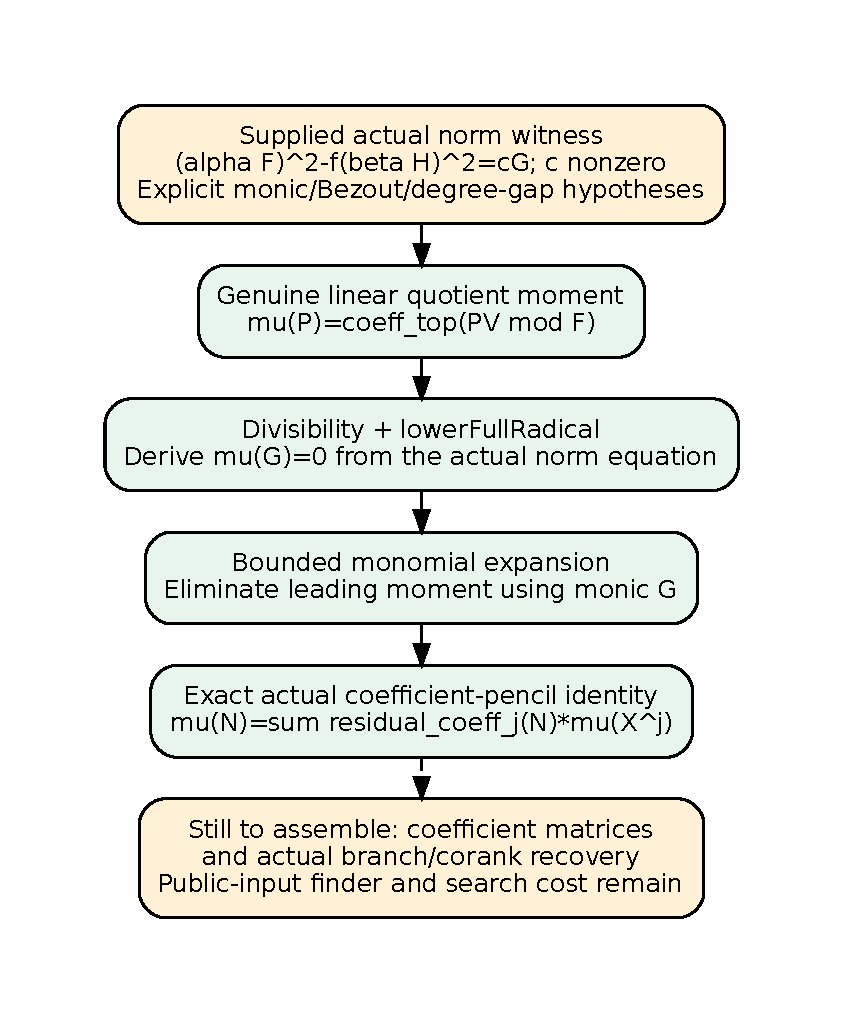
\includegraphics[width=0.9\linewidth,height=0.36\textheight,keepaspectratio]{pencil.pdf}
\end{center}

\newpage
{\Large Proof map, checks and remaining dependencies}

\textbf{Source.} \path{NormPencilFunctional.lean}, frozen source commit
\path{78123b01d}. Definitions and declarations:
\path{moment}, \path{momentApply}, \path{annihilatesTarget},
\path{coefficientExpansion}, \path{coefficientPencil},
\path{normCoefficientPencil}, \path{normPolarization}.
Five substantive interpretive PCC records are unsigned; exact declaration
hashes and scope are retained. Earlier CRT/radical/moment hashes are unchanged.

\textbf{Checks.} Lean4.35.0, unchanged pinned CryptoLean and Mathlib.
Build004 passes3147 jobs. Final tracked-source gate covers110 declarations,
zero failing and zero additional trusted axioms. Fresh kernel replay including
imports exits0. Standard foundations only: \path{propext},
\path{Classical.choice}, \path{Quot.sound}. No signed PCC standing is claimed.

Build001 failed on exported definitional-equality visibility of the new
functional; an explicit simp proof resolves it. Build003 failed the missing
import of the reused degree theorem; its actual module is now imported.
Build002 was successful at the pre-specialization scope. All logs, including
failed attempts, are preserved in the evidence directory.

\textbf{Native identity.} The universal commutative-ring polarization is
\[
 \operatorname{Norm}(A+Q,B+T)-\operatorname{Norm}(A,B)
 -\operatorname{Norm}(Q,T)=2(AQ-fBT).
\]
Native record \path{IDC1h345f3824264d232a}, with32 statement-derived and32
extra-stream points, pins this exact universal Lean source. The maintained
issuer/checker is unchanged. Its adapter's22 inherited tests pass, including
tamper/statement-swapping controls. It does not execute Lean or establish the
conditional coefficient-pencil theorem. Division by2 is not used here.

\textbf{Next.} Define actual bounded coefficient bases and derive matrix
pencil equality from the functional identity. Instantiate the branch lemma,
compute the scaled witness-line intersection, then transfer its dimension to
corank1 and guarded adjugate recovery. Constant/degree-drop charts and a
public-input finder remain separate. The required $2^{o(n)}$ bit search cost,
$n=\lceil\log_2r\rceil$, does not follow from certificate existence.

\textbf{Earlier completion proposal.} The nonscalar origin/jet-completion
idea motivated this rank-directed certificate design. These identities do not
prove reachability through $W_{\rm base}+C(T)H(T)$ or provide an efficient
choice of its free coefficients.

\textbf{Sources and resources.} Previous matrix-bridge plan and exact pinned
\path{Polynomial.RingDivision} scalar-remainder/linear-map declarations,
\path{Degree.Support} bounded monomial expansion, prior degree bound and
lower radical. KB and conductor unavailable; bounded fallback recorded, no
priority claim for these classical ingredients. No paid job, empirical
runtime/scaling campaign or budget override. Monthly isolab budget exhausted.
No benchmark, leaderboard or ecdb changes. The source-linked Markdown report,
editable DOT/SVG, diagram PDF and evidence accompany this PDF.
\end{document}
